\chapter{Implementation}
\label{chaptImplementation}
In this chapter, we describe the implementation of our demonstration game and explain the basic principles and algorithms behind it. Then we present measurements of performance of main algorithms used in the implementation.

At first, we considered implementation based on \emph{A fast method for simulating destruction and the generated dust and debris} (FMSDGDD) (see \cref{sec:edem}). However, after degrading performance issues~\cref{sec:testing} we decided to abandon this approach.

After consideration of various approaches implemented in games and also proposed efficient solutions to the problem of real-time destructible environment, we decided to implement and test an approach based on \emph{Geomod} (described in \cref{sec:common}) technique. The \emph{Geomod} inspired us to create object representing empty space and use boolean subtraction operation on the mesh to generate damaged body. Abandoned FMSDGDD approach influenced us to generate debris equivalent to the removed volume and use boolean intersection. We implemented this idea by using an intersection of \emph{Geomod} inspired empty space and original mesh as a debris.

\section{Main algorithm}
As mentioned, our algorithm uses boolean operations similarly to \emph{Geomod}s removal of an empty space from the terrain. The difference is that we apply this method to rigid body objects and permanently alter their mesh. The shape of removed object is determined by Voronoi cell that is generated dynamically for every collision. The collision information is received from the physics engine.

Our approach generates Voronoi cell at the point of collision. The decision to use one cell instead of a fracture pattern, like the one described in Real Time Dynamic Fracture with Volumetric Approximate Convex Decompositions algorithm (see \cref{sec:RTDF}), is based on the fact that we want to observe how dependent is our design on the complexity of destructed objects and not on the complexity of fracture pattern. Our implementation is easily expandable to the use of multiple cells or cells of any shape. 

After the cell generation, the difference of original mesh and the Voronoi cell is calculated to represent the damaged objects. To generate the debris, the intersection of original mesh and the Voronoi cell is calculated. This action effectively cuts the object into two or more pieces, all of which are put back into simulation and can be damaged again (see \cref{fig:subtraction}). The Voronoi cell was chosen because it has easily randomizable shape and provides aesthetically good results.

The cost of fracturing in our implementation is solely dependent on the size and complexity of the fractured object~\cref{sec:testing}. This makes the method suitable for use in computer games with a large number of simple objects with low polygon meshes.

\begin{figure}
        \centering
        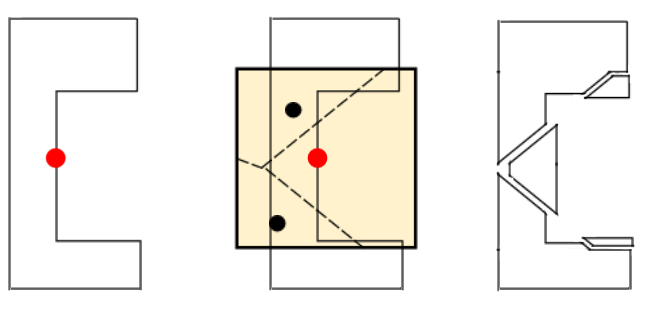
\includegraphics[width=\textwidth]{img/subtractionProcess}
        \caption{object with point of collision (left), generated Voronoi cells (centre), object divided into five new smaller objects after subtraction of the Voronoi cell belonging to the point of collision (right)}
        \label{fig:subtraction}
\end{figure}

To generate the Voronoi cell, we create a closed domain with the centre at the point of collision. In the domain, we need to create random points so the Voronoi cell of the point of collision does not cover entire domain. This step also ensures variability of generated cells. After that, we can use a Voronoi cell belonging to the point of collision as the object we subtract from the object being damaged. The boundaries of the domain clip the generated Voronoi cell, therefore the Voronoi cell can never be larger than the domain. Randomization of the size and shape of a Voronoi cell guarantees different result after every damage application.

\section{Program Structure}
The program is structured into four main components, Physics, Graphics, Controllers and Mesh Manipulation (see~\cref{fig:architecture}). Physics performs rigid body simulation and detects collisions. Graphics is used as a output device. Controllers contain the core of the application and process user input. Mesh Manipulation is the part of the application that handles the destruction of the environment.
\begin{figure}
        \centering
        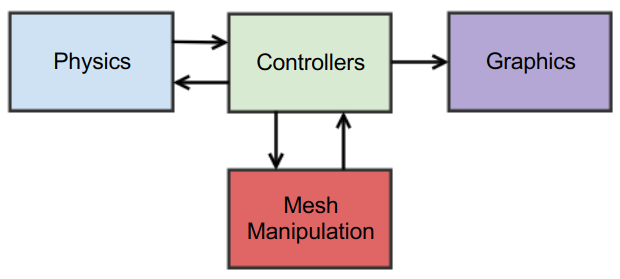
\includegraphics[width=0.7\textwidth]{img/architecture}
        \caption{Diagram showing architecture of the application}
        \label{fig:architecture}
\end{figure}

\label{sec:structure}
The main program loop runs in following steps:
\begin{enumerate}
\item Perform a step in physics simulation.
\item Handle collisions and perform destruction, as described in  \cref{sec:collisions}.
\item Read user input and then apply correct forces to the controlled vehicle.
\item Render the current state of objects. In this step, a graphical representation of every object is updated to comply with its rigid body version.
\end{enumerate}

\begin{figure}
        \centering
        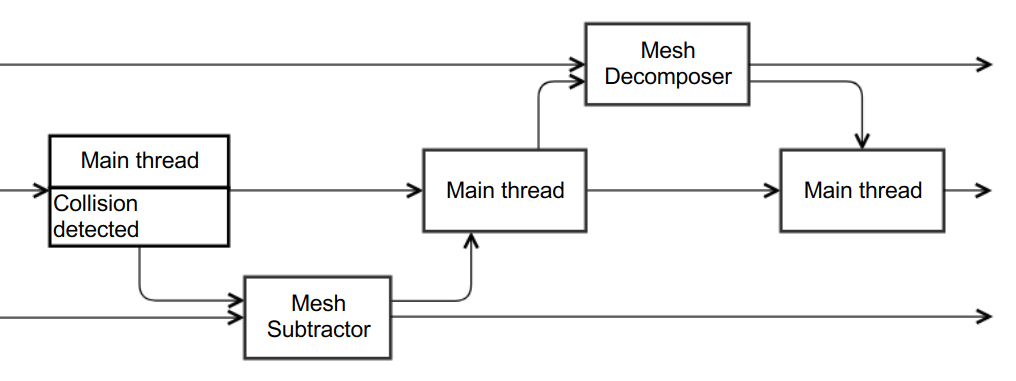
\includegraphics[width=\textwidth]{img/decompositionFlow}
        \caption{Diagram is showing multiple threads handling collision event. }
        \label{fig:threads}
\end{figure}

We want to keep a constant frame-rate in our application, but we do not  expect the mesh subtraction and convex decomposition tasks to perform in required time and therefore we execute them asynchronously in separate threads. As a result, the program is running in three threads (\cref{fig:threads}): the main thread, a thread for subtracting meshes and a thread for decomposing triangular mesh into a set of convex shapes (\cref{sec:decomposition}). Both subtraction and decomposition threads communicate solely with the main thread, and all communication is done in producer-consumer model. Figure \ref{fig:objectInThreads} shows the changes of the object and its collision shape across all threads.

We use only one thread for all mesh subtraction tasks because we anticipate that the most of the consecutive collisions are going to be triggered by the same object --- shooting at one building multiple times in a row. In this situation, one subtraction does not have valid input data until the previous one has finished, which leads to sequential processing. If we were to expect the collision occurring randomly on independent objects we could implement a thread pool for resolving subtraction tasks. When processing multiple collisions on the same object with multiple threads, the order of applying subtraction is not important as long as all tasks are processed and applied. Multiple thread solution would require implementation of a locking mechanism to avoid race conditions.

A use of a larger thread pool could be useful for convex decomposition. With multiple threads, the object could have been changed since the current calculation started. This conflicting state means we can not apply the current result but we know for sure that another decomposition task was created when the change occurred. We do not know whether the newer task has already finished or not, but we know for certain, that if we discard our decomposition, the object has either temporary shape or a new valid decomposition. We did not implement a thread pool solution because we did not see it necessary and our hardware \todo{current common gaming hardware, citation needed} is not well suited for running more than four simultaneous threads.

\begin{figure}
        \centering
        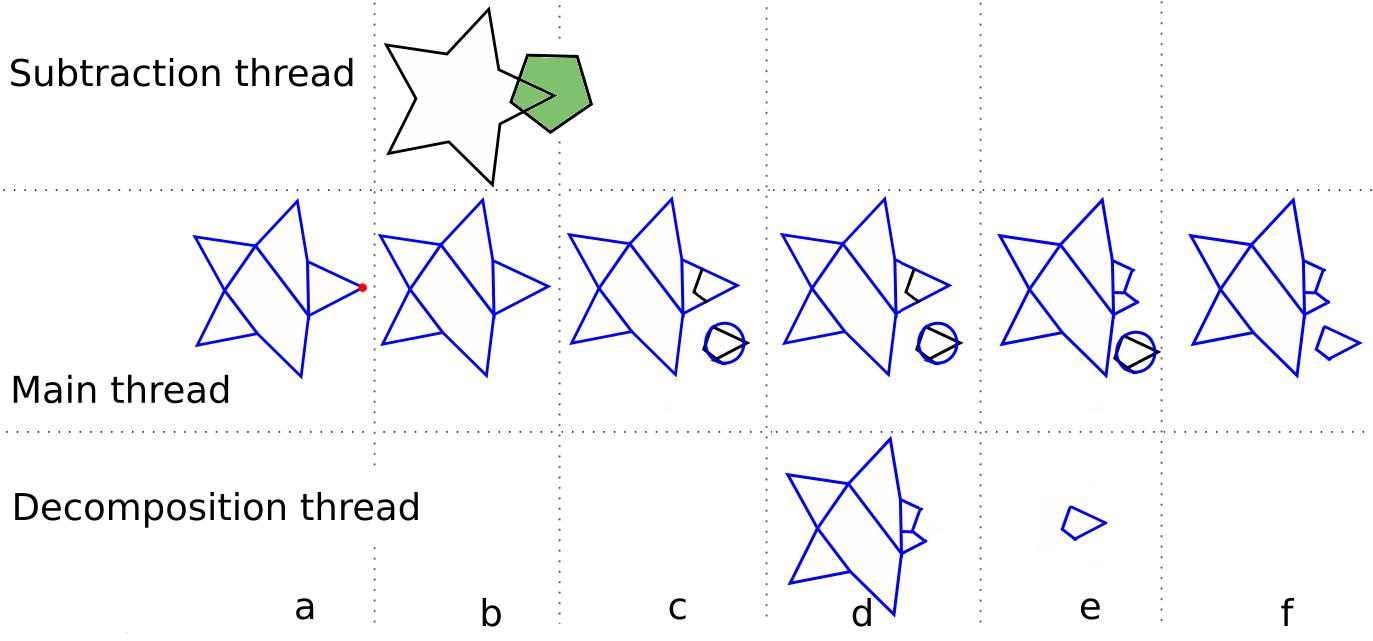
\includegraphics[width=\textwidth]{img/object-progress}
       \caption{Simplified overview of collision handling across multiple threads in simultaneous time slots. (a): collision was detected (red), (b): Voronoi cell (green) is being subtracted from the original mesh (black) in subtraction thread, (c): the result of the subtraction are two objects --- one one without change in collision shape (blue) and one with temporary spherical shape, (d) and (e): new collision shapes are computed in decomposition thread, (f): the final result.}
        \label{fig:objectInThreads}
\end{figure}

\section{Collision handling}
\label{sec:collisions}
After the detection of collision, physics engine gives us a reference to two rigid bodies participating in that collision, point of collision and vector of applied impulse. For simplification, we consider only one object, the point of impact and the force. The second object is processed symmetrically.

Some collisions can be results of an object placed on ground or collisions with not enough force to damage the object. We need to filter out those unwanted collisions.

For every collision that is selected as acceptable for damaging the object, we generate Voronoi cell as described before, and move meshes of both objects into a task for mesh subtraction thread. After enqueuing all collisions, we check if there are any prepared subtraction results for further use. The result of one subtraction task is a set of meshes that represent new objects. For every mesh, we create a new incomplete object without its convex decomposition that is needed for the physics engine to perform accurate collision detection. Because the decomposition can take relatively long, we create a simple temporary collision shape, we decided to use a sphere for the new objects and keep using original \todo{Jak poznas kterej objekt je novej a kterej je original? je prvy v poli :D} collision shape for the original object. Then we create tasks for decomposition of current meshes into new collision shapes and proceed with simulation, not waiting for the result. Decomposition is done in a separate thread and the result is returned to the main thread where decomposition results are applied to objects --- temporary shape is replaced by compound shape consisting of convex parts.

This process guarantees that we do not wait for either subtraction or decomposition and therefore we can have stable fps in our game.  It is better for the gameplay to have stable fps and lag behind with the simulation because poor performance in the main loop of the games makes the game stuttering. Meanwhile, a destruction happening a few frames later can be covered in animations of dust. To ensure consistent behaviour of new objects (we can put them into the simulation, and they do not fall through each other or otherwise not comply with laws of physics) when using a temporary collision shape, we need to make the temporary shape resemble the mesh as much as possible.  For the already existing objects keeping the older collision shape for a while longer should not disturb the simulation as the closest objects to this space are a newly generated object, those should be thrown away from the point of collision either way. For the new object, we use the sphere with the diameter equal to the shortest edge of the objects bounding box, meaning that the newly created objects have smaller collision shapes than meshes. The experiments showed that this factor does not visually impact simulation and the presence of the collision shape ensures that the object will not fall through other objects. 


\section{Convex Decomposition}
\label{sec:decomposition}
Regardless of used physics engine, our objects are represented as triangular meshes. Implementing mesh to mesh collisions is possible, but highly impractical. Even if checking every vertex of one mesh against all vertices of second mesh is sufficient, the complexity of algorithm would be dependent on the number of vertices.

To be able to perform mesh to mesh collisions with complexity independent on triangle count, we must find a way to describe the object as a set of geometrically simpler shapes. The convex shapes are the easiest for detecting mutual intersections, but encapsulating whole mesh into a convex hull would produce imprecise collisions. This problem is solved by performing a convex decomposition. Convex decomposition process splits the input object into a set of convex shapes, forming a compound shape. Now the complexity of the collision algorithm depends on the number of convex parts. The size of convex decomposition is dependent on the number of concave features on decomposed mesh.

While the exact convex decomposition can still produce a significant number of convex parts~\cite{convexDecomp}, in the setting of a computer game, the speed of calculation is much more relevant than the precision --- small differences between collision shapes and visual meshes are not considered to be a problem. To be able to perform collision detection at real-time, many approximate convex decomposition algorithms that sacrifice some precision to gain performance have been proposed. One of those algorithms is \emph{Hierarchical Approximate Convex Decomposition} algorithm (see \cref{sec:decompositionLib}) which we decided to use.

\section{Measurements and experiments}
\label{sec:testing}
In this section we show the conducted experiments with the goal of evaluating efficiency our approach. 

To gather the data, we added special code that dumps the timing from the program and we also prepared input files for testing. We are interested in the times of two most complicated tasks in our application, mesh subtraction and convex decomposition. 

Data are dumped into \emph{data/} folder. Three files are present in the folder, one contains the dump of the times it took to resolve subtraction tasks, one does the same for decomposition tasks and the third one contains total times it took for the single object to get from being put into subtraction queue until new decomposition is applied.

We designed two different experiments, the performance test to measure the behaviour of our our approach in the world with multiple objects and fast sequences of collisions and the mesh complexity test to identify relation between number of number of triangles and subtraction/decomposition.

\subsection{Performance test}
For a performance test we prepared a world configuration (copy in \emph{performance\_test.cfg}) consisting of objects with models, counts and geometric complexity specified in \cref{tab:objects}.
We recorded about 2000 collisions by repeatedly shooting the buildings at random locations. Recorded data can be seen in \cref{fig:boxtimes}.

\begin{table}
 	\centering
\begin{tabular}{lrr}
  Model & Count & Triangles \\
  \hline
  \texttt{media/building.obj} & 7 & 60 \\
  \texttt{media/missile.obj} & 1 & 142 \\
  \texttt{media/ship.obj} & 1 & 104
\end{tabular}
\caption{Objects and their complexities used in the measurement.}
	\label{tab:objects}
\end{table}

\begin{figure}
\centering
\begin{tikzpicture}
  \begin{axis}
    [
    boxplot/draw direction=x,
    ytick={1,2,3},
    yticklabels={Subtraction, Decomposition, Overall Time},
    height=4cm,
    width=10cm,
    xlabel=Time (s),
    ]
    \addplot+[
    boxplot prepared={
      median=0.14,
      upper quartile=0.24259,
      lower quartile=0.091783825,
      upper whisker=0.46,
      lower whisker=0.03
    },
    ] coordinates {};
    \addplot+[
    boxplot prepared={
      median=0.114929,
      upper quartile=0.1292675,
      lower quartile=0.1094205,
      upper whisker=0.16,
      lower whisker=0.10
    },
    ] coordinates {};
    \addplot+[
    boxplot prepared={
      median=0.303041,
      upper quartile=0.41976,
      lower quartile=0.2415265,
      upper whisker=0.7,
      lower whisker=0.05
    },
    ] coordinates {};
  \end{axis}
\end{tikzpicture}
\caption{Box plot showing the distribution of the duration in seconds (horizontal axis) of given task (vertical axis)}
\label{fig:boxtimes}
\end{figure}



Our expectation is that a delay shorter than around 300ms between the collision and rendering of its resulting objects would be acceptable for a game, and that the separate threads would ensure that this delay would not impact the frame rate. The experiment confirms that on given input we can successfully meet this expectation.

The problem seems to by a high variance in overall time of the whole process starting with mesh subtraction and ending at applying convex decomposition. This can be explained by the tasks waiting in the queue for processing and shows that our solution is not well suited for a fast sequence of collisions. The problem here is that after every collision only one subtraction task is created, but the number of decompositions is nondeterministic and depends on the shape of the destructed object, the generated Voronoi cell and the position of the collision. Use of a thread pool with more advanced bookkeeping of the decomposition dependencies would aid in solving that problem (proposed in ~\cref{sec:structure}).

\subsection{Performance impact of mesh complexity}
We designed an experiment to measure a relationship between a number of triangles and time required to complete the two already measured tasks. The collected data are subtraction time and convex decomposition time. For the experiment we prepared five cubes with same size but with different number of triangles in their mesh. We created an isolated environment with only one cube placed in it and then executed the application to collect the data. The data were generated as a result of a collision after the cube dropped on to the ground. The experiment was repeated with each of the prepared cubes and run multiple times to collect a larger sample for statistical analyses. The results of the experiment are shown in \cref{tab:subtraction-decomposition} . 
\begin{table}
\centering
\begin{tabular}{r r r}
\# triangles & subtraction & decomposition \\
\hline
12 & 0.037 & 0.118 \\
108 & 0.069 & 0.135 \\
588 & 0.134 & 0.261 \\ 
2700 & 0.386 & 2.362 \\ 
10092 & 1.211 & 12.007 \\
\end{tabular}
\caption{Average time (in seconds) of processing the given task with the given number of triangles in the mesh. All data are collected on the same cube with only difference in number of triangles.}
\label{tab:subtraction-decomposition}
\end{table}

\begin{figure}
\centering
\begin{tikzpicture}
  \begin{axis}
    [
	boxplot/draw direction=x,
    ytick={1,2,3,4},
    yticklabels={12, 108, 588, 2700},
    ylabel=\# triangles,
    xlabel=Time (s),
    width=12cm,height=5cm,
    tick label style={/pgf/number format/fixed},
    ]
    \addplot+[
    boxplot prepared={
      median=0.03609005,
      upper quartile=0.039086475,
      lower quartile=0.0343537,
      upper whisker=0.05,
      lower whisker=0.03
    },
    ] coordinates {};
    
    \addplot+[
    boxplot prepared={
      median=0.06526395,
      upper quartile=0.070043275,
      lower quartile=0.064723875,
      upper whisker=0.070043275,
      lower whisker=0.06
    },
    ] coordinates {};
    \addplot+[
    boxplot prepared={
      median=0.1335775,
      upper quartile=0.1341765,
      lower quartile=0.13317175,
      upper whisker=0.14,
      lower whisker=0.13
    },
    ] coordinates {};
    
    \addplot+[
    boxplot prepared={
      median=0.384889,
      upper quartile=0.391104,
      lower quartile=0.38266425,
      upper whisker=0.4,
      lower whisker=0.38
    },
    ] coordinates {};
  \end{axis}
\end{tikzpicture}
\caption{Relation between number of triangles and time required for subtraction task.}
\label{fig:triangletimes}
\end{figure}

\begin{figure}
\centering
\begin{tikzpicture}
  \begin{axis}
    [
	boxplot/draw direction=x,
    ytick={1,2,3,4},
    yticklabels={12, 108, 588, 2700},
    ylabel=\# triangles,
    xlabel=Time (s),
    width=12cm,height=5cm,
    tick label style={/pgf/number format/fixed},
    ]
    \addplot+[
    boxplot prepared={
      median=0.112423,
      upper quartile=0.12278675,
      lower quartile=0.1105495,
      upper whisker=0.12278675,
      lower whisker=0.11
    },
    ] coordinates {};
    
    \addplot+[
    boxplot prepared={
      median=0.133383,
      upper quartile=0.14062125,
      lower quartile=0.128652,
      upper whisker=0.1512,
      lower whisker=0.127272
    },
    ] coordinates {};
    \addplot+[
    boxplot prepared={
      median=0.2534035,
      upper quartile=0.27878175,
      lower quartile=0.24843475,
      upper whisker=0.288963,
      lower whisker=0.246148
    },
    ] coordinates {};
    
    \addplot+[
    boxplot prepared={
      median=2.333265,
      upper quartile=2.428165,
      lower quartile=2.282675,
      upper whisker=2.56834,
      lower whisker=2.27192
    },
    ] coordinates {};
  \end{axis}
\end{tikzpicture}
\caption{Relation between number of triangles and time required for convex decomposition task.}
\label{fig:decomtimes}
\end{figure}

The experiment showed us the limits of our approach. For the mesh subtraction, we can tolerate meshes with the size of about 2000 triangles (see \cref{fig:triangletimes}).  On the other hand, as shown on~\cref{fig:decomtimes}, convex decomposition times grow significantly faster and reaches 300ms the second somewhere around 1000 triangles.


\subsection{Testing the concept of EDEM}
To test EDEM (described in \cref{sec:edem}), we set up a cube divided into 439 tetrahedrons. After introducing constraints to hold the tetrahedrons together, we experienced a drop from 60fps (set as an upper limit) to 13fps. Having a large number of elements connected with springs in the simulation can also trigger an undesirable behaviour, such as contractions, retractions and self-induced explosions of the object. Performance issues and problems with keeping elements in a stable state concluded that the approach was not suitable for our implementation.




